\documentclass{article}
\usepackage{xeCJK}
\usepackage[utf8]{inputenc}
\usepackage{graphicx}
\usepackage{soul}
\usepackage{caption}
\usepackage[utf8]{inputenc}
\usepackage{amsmath}
\usepackage[dvipsnames]{xcolor}
\DeclareMathOperator*{\argmax}{arg\,max}
\DeclareMathOperator*{\argmin}{arg\,min}

\title{How to train neural network}
\author{Yun-Hsiang Chan}
\date{June 2021}

\begin{document}

\maketitle

Neural Network Training Loop, See Figure 1.

\begin{figure}
    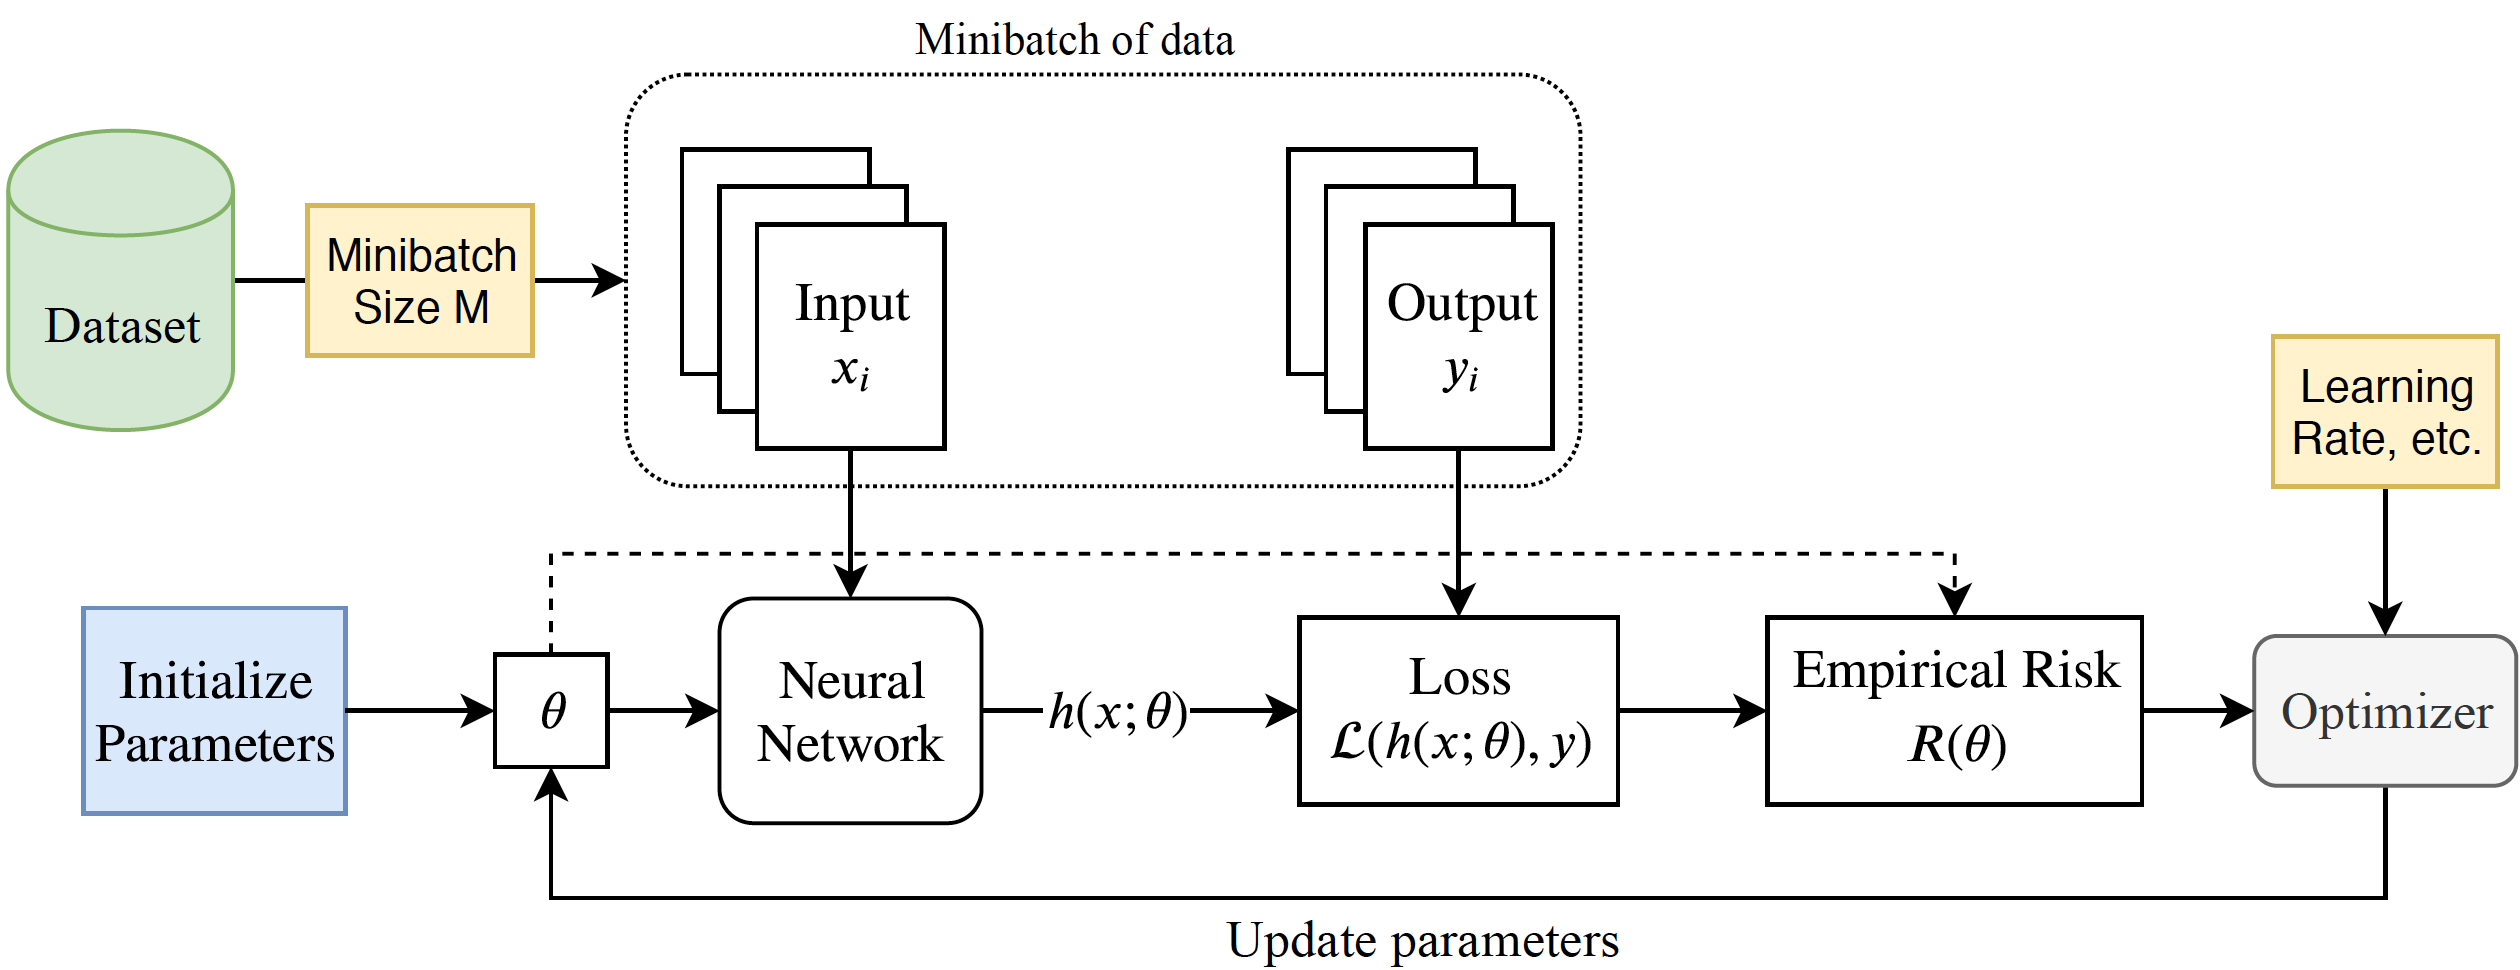
\includegraphics[width = 15cm]{Tut03_TrainDiag.png}
    \caption{Neural Network Training Loop}
\end{figure}

\section*{I. Initialization of Parameters} 
- Idea 1: Constant Initialization \\
Result: identical gradients, identical neurons, bad! \\
\\
- Idea 2: Random weights, to break symmetry \\
Too \textbf{large} of initialization $\Rightarrow$ \textbf{exploding gradient} \\
Too \textbf{small} of initialization $\Rightarrow$ \textbf{vanisihing gradient} \\
\\
Two Popular schemes: \\
1. \textbf{Xavier} Init: For $Tanh$ activation \\
$$W^{[l]} \sim N(\mu = 0, \sigma^2 = \frac{1}{n^{[l-1]}}), b^{[l]} = 0$$
or, 
$$W^{[l]} \sim N(0, \frac{2}{n^{[l-1]} + n^{[l]}}), b^{[l]} = 0$$
\\
2. \textbf{Kaiming He} Init: For \textbf{ReLU} activation \\
$$W^{[l]} \sim N(\mu = 0, \sigma^2 = \frac{2}{n^{[l-1]}}), b^{[l]} = 0$$
\\
\textbf{Note:} $n^{[l]}$ is the number of neurons in a layer, $l$ is layer

\subsection*{1.1 Xavier Initialization Intuition}
1. \textbf{Variance} of activation approximately \textbf{constant} across every layer
$$Var(a^l) = Var(a^{l-1})$$
2. \textbf{Mean} of the activation and weights = \textbf{zero}
$$E[w^l] = 0, E[a^l] = 0$$

\section*{II. Batch Normalization Layer}
Can we compensate for bad initializations in some other ways? \\
\\
\textbf{BatchNorm's Idea} \\
- Explicitly normalize the activations of each layer to be unit Gaussian \\
- Apply immediately after fully connected/con layers and before non-lineraities \\
- Learn an additional scale and shift and running statisitcs for test time \\
- Significantly speeds up training in practice \\
- Distribution after connected layer is much more stable with BN, reducing the "internal covariate shift", i.e. the change in the distribution of network activations due to the change in network parameters during training. 

\section*{III. Optimization}
Given a training set, we have prediction function and loss function. We want to find the parameters that minimize the empirical risk. \\
\\
\textbf{- Batch Grdient Desccent} \\
\\
\textbf{- Stochastic Gradient Descent} \\
\\
\textbf{- Gradient Descent with Momentum} \\
Pros: acclerate learning by accumulating some "velocity/momentum" with the past gradients \\
\\
\textbf{- Nesterov Accerlated Gradient} \\
Pros: look into the future to see how much momentum is required. 

\section*{IV. Learning Rate Schedulers}
We adjust the learning rate in our learning process. \\
\\
\textbf{- Adagrad} \\
Intuition: It increases the learning rate for more sparse features and decreases the learning rate for less sparse ones, according to the history of the gradient. \\
\\
\textbf{- RMSprop/Adadelta} \\
Intuition: Unlike Adagrad, the denominator places a significant weight on the most recent gradient. This also helps avoid decreasing learning rate too much. \\
\\
\textbf{- Adam} \\
The most popular way, combining Ada and RMSprop.

\section*{V. Learning Rate Schedule}
- A good learning rate should not be too big or too small. \\
\\
Find a decay schedule for it. \\
\textbf{- Step Decay} \\
\textbf{- Exponential Decay} \\
\textbf{- 1/t decay}

\section*{VI. Batch Size}
Typically, small batches are power of $2$: $32, 64, 128, 256, 512$ \\
\\
\textbf{Large} Batch Size has: \\
\textbf{- Fewer Frequency of updates} \\
\textbf{- More accurate} gradient \\
\textbf{- More paralleization} efficiency \\
\textbf{- May hurt generalization}

\section*{VII. Hyperparameter Tuning}
Grid search and Random search.



\end{document}